\section{System Architecture and Design Philosophy}

The architecture of Open Deep Search embodies a fundamental design philosophy prioritizing modularity, extensibility, and model-agnostic integration. This section examines the core architectural patterns that enable the system to achieve competitive performance while maintaining the flexibility essential for research advancement and practical deployment across diverse use cases. The design reflects careful consideration of the trade-offs between simplicity and capability, between optimization for specific models and generalization across the rapidly evolving landscape of language models, and between immediate performance and long-term adaptability.

\subsection{Core Design Principles}

The architectural foundation of Open Deep Search rests on several interconnected design principles that distinguish it from both proprietary alternatives and earlier open-source implementations. Understanding these principles provides essential context for evaluating specific technical decisions documented in subsequent sections.

The principle of radical modularity governs component design throughout the system. Rather than implementing a monolithic architecture where search capabilities and reasoning logic exist as tightly coupled elements, Open Deep Search separates functionality into discrete components with well-defined interfaces. The Open Search Tool operates as an independent module responsible for all aspects of information retrieval, from query understanding through result augmentation. The Open Reasoning Agent exists as a separate component that orchestrates tool usage and synthesizes information. This separation enables independent development and optimization of each component, facilitates testing and debugging by isolating failure modes, and allows selective deployment where only certain capabilities are required.

The commitment to model agnosticism represents a strategic architectural decision with far-reaching implications. Open Deep Search deliberately avoids optimization for any specific base language model, instead providing a plug-and-play integration framework that accepts any model accessible through the LiteLLM unified interface. This design choice acknowledges the rapid pace of language model development where state-of-the-art capabilities shift between model families on timescales of months rather than years. By decoupling system capabilities from specific model implementations, Open Deep Search creates a sustainable architecture that improves automatically as better base models become available. Users can select models based on their specific requirements balancing performance, cost, latency, and privacy considerations without requiring system modifications.

The architectural emphasis on transparency and debuggability reflects the open-source ethos while providing practical benefits for system development and deployment. Every component exposes internal state and reasoning traces, enabling detailed analysis of system behavior. The ReAct agent implementation makes reasoning explicit through structured thought-action-observation loops that can be inspected to understand decision-making processes. The CodeAct agent generates human-readable Python code that documents exactly how the system approaches query resolution. This transparency serves multiple purposes including facilitating research on reasoning patterns, enabling rapid diagnosis of failures, supporting customization for domain-specific requirements, and building user trust through explainability.

The design principle of graceful degradation ensures system robustness in the face of component failures or resource constraints. Rather than failing catastrophically when individual components encounter errors, Open Deep Search implements fallback mechanisms at multiple levels. When the primary ReAct reasoning approach fails to produce satisfactory results, the system automatically falls back to Chain-of-Thought Self-Consistency that generates multiple candidate answers and selects the most consistent response. When web scraping encounters errors during augmentation, the system continues operation using search engine result page snippets. When external API services become unavailable, the system can operate with reduced capabilities rather than complete failure. This defensive architecture improves reliability for production deployment while maintaining performance under ideal conditions.

The commitment to computational efficiency balanced against capability drives numerous implementation decisions. Open Deep Search avoids unnecessary computation through mechanisms like caching of search results, reuse of embeddings across queries, and adaptive search strategies that vary effort based on query complexity. The system supports both default and pro modes that trade latency against accuracy, enabling users to select appropriate operating points for their applications. The architecture accommodates resource-constrained deployments through support for model quantization, flexible infrastructure requirements, and scalable component deployment.

\subsection{Two-Component Architecture}

The high-level architecture of Open Deep Search comprises two primary components that work in concert to transform user queries into comprehensive, factually grounded responses. This division of responsibilities reflects a clean separation of concerns where information retrieval and reasoning operate as distinct but complementary capabilities.

The Open Search Tool implements all functionality related to finding and processing information from external sources. This component accepts natural language queries and returns structured context comprising relevant information gathered from the web. The tool encapsulates three sequential stages of processing. Query rephrasing expands the original user query into multiple related queries that increase the diversity and coverage of retrieved information. Retrieval executes searches using either the Serper.dev API or self-hosted SearXNG instances, collecting search engine result pages with associated metadata including titles, URLs, descriptions, and publication dates. Augmentation optionally enhances results through web scraping, content chunking, semantic embedding, and reranking to select the most relevant passages. The output from the Open Search Tool provides rich contextual information that subsequent reasoning components can leverage to formulate answers.

The Open Reasoning Agent orchestrates the overall query resolution process, deciding when to invoke the search tool, how to interpret retrieved information, and how to synthesize comprehensive responses. The agent operates as a decision-making component that can invoke multiple tools including the Open Search Tool for information retrieval, Wolfram Alpha integration for mathematical computation, and recursive thinking capabilities for complex reasoning. The agent maintains conversation state, tracks the progress of multi-step reasoning, and determines when sufficient information has been gathered to answer the query. Two distinct agent implementations provide different approaches to this orchestration challenge, offering trade-offs between interpretability, performance, and flexibility.

The interaction between these components follows a clearly defined protocol. User queries enter the system and are processed initially by the reasoning agent, which assesses what information is required to formulate a response. The agent generates appropriate tool invocations, typically beginning with searches via the Open Search Tool. Retrieved context returns to the agent, which analyzes the information to determine whether sufficient knowledge has been gathered. For simple queries, a single search cycle may suffice. For complex multi-hop queries, the agent may iteratively refine its understanding, generate follow-up searches, and progressively build toward a complete answer. Throughout this process, the agent maintains explicit reasoning traces that document its decision-making, providing transparency into how conclusions were reached.

This two-component architecture provides several advantages over monolithic alternatives. The clean separation enables independent optimization where search capabilities can improve without modifying reasoning logic and vice versa. The modular design facilitates testing where each component can be validated in isolation before integration testing of the complete system. The architecture supports flexible deployment configurations including standalone search tool usage for applications not requiring full reasoning capabilities, integration of the search tool into existing agent frameworks beyond those provided by Open Deep Search, and deployment of reasoning agents with alternative tool suites for specialized domains.

\begin{figure}[htbp]
    \centering
    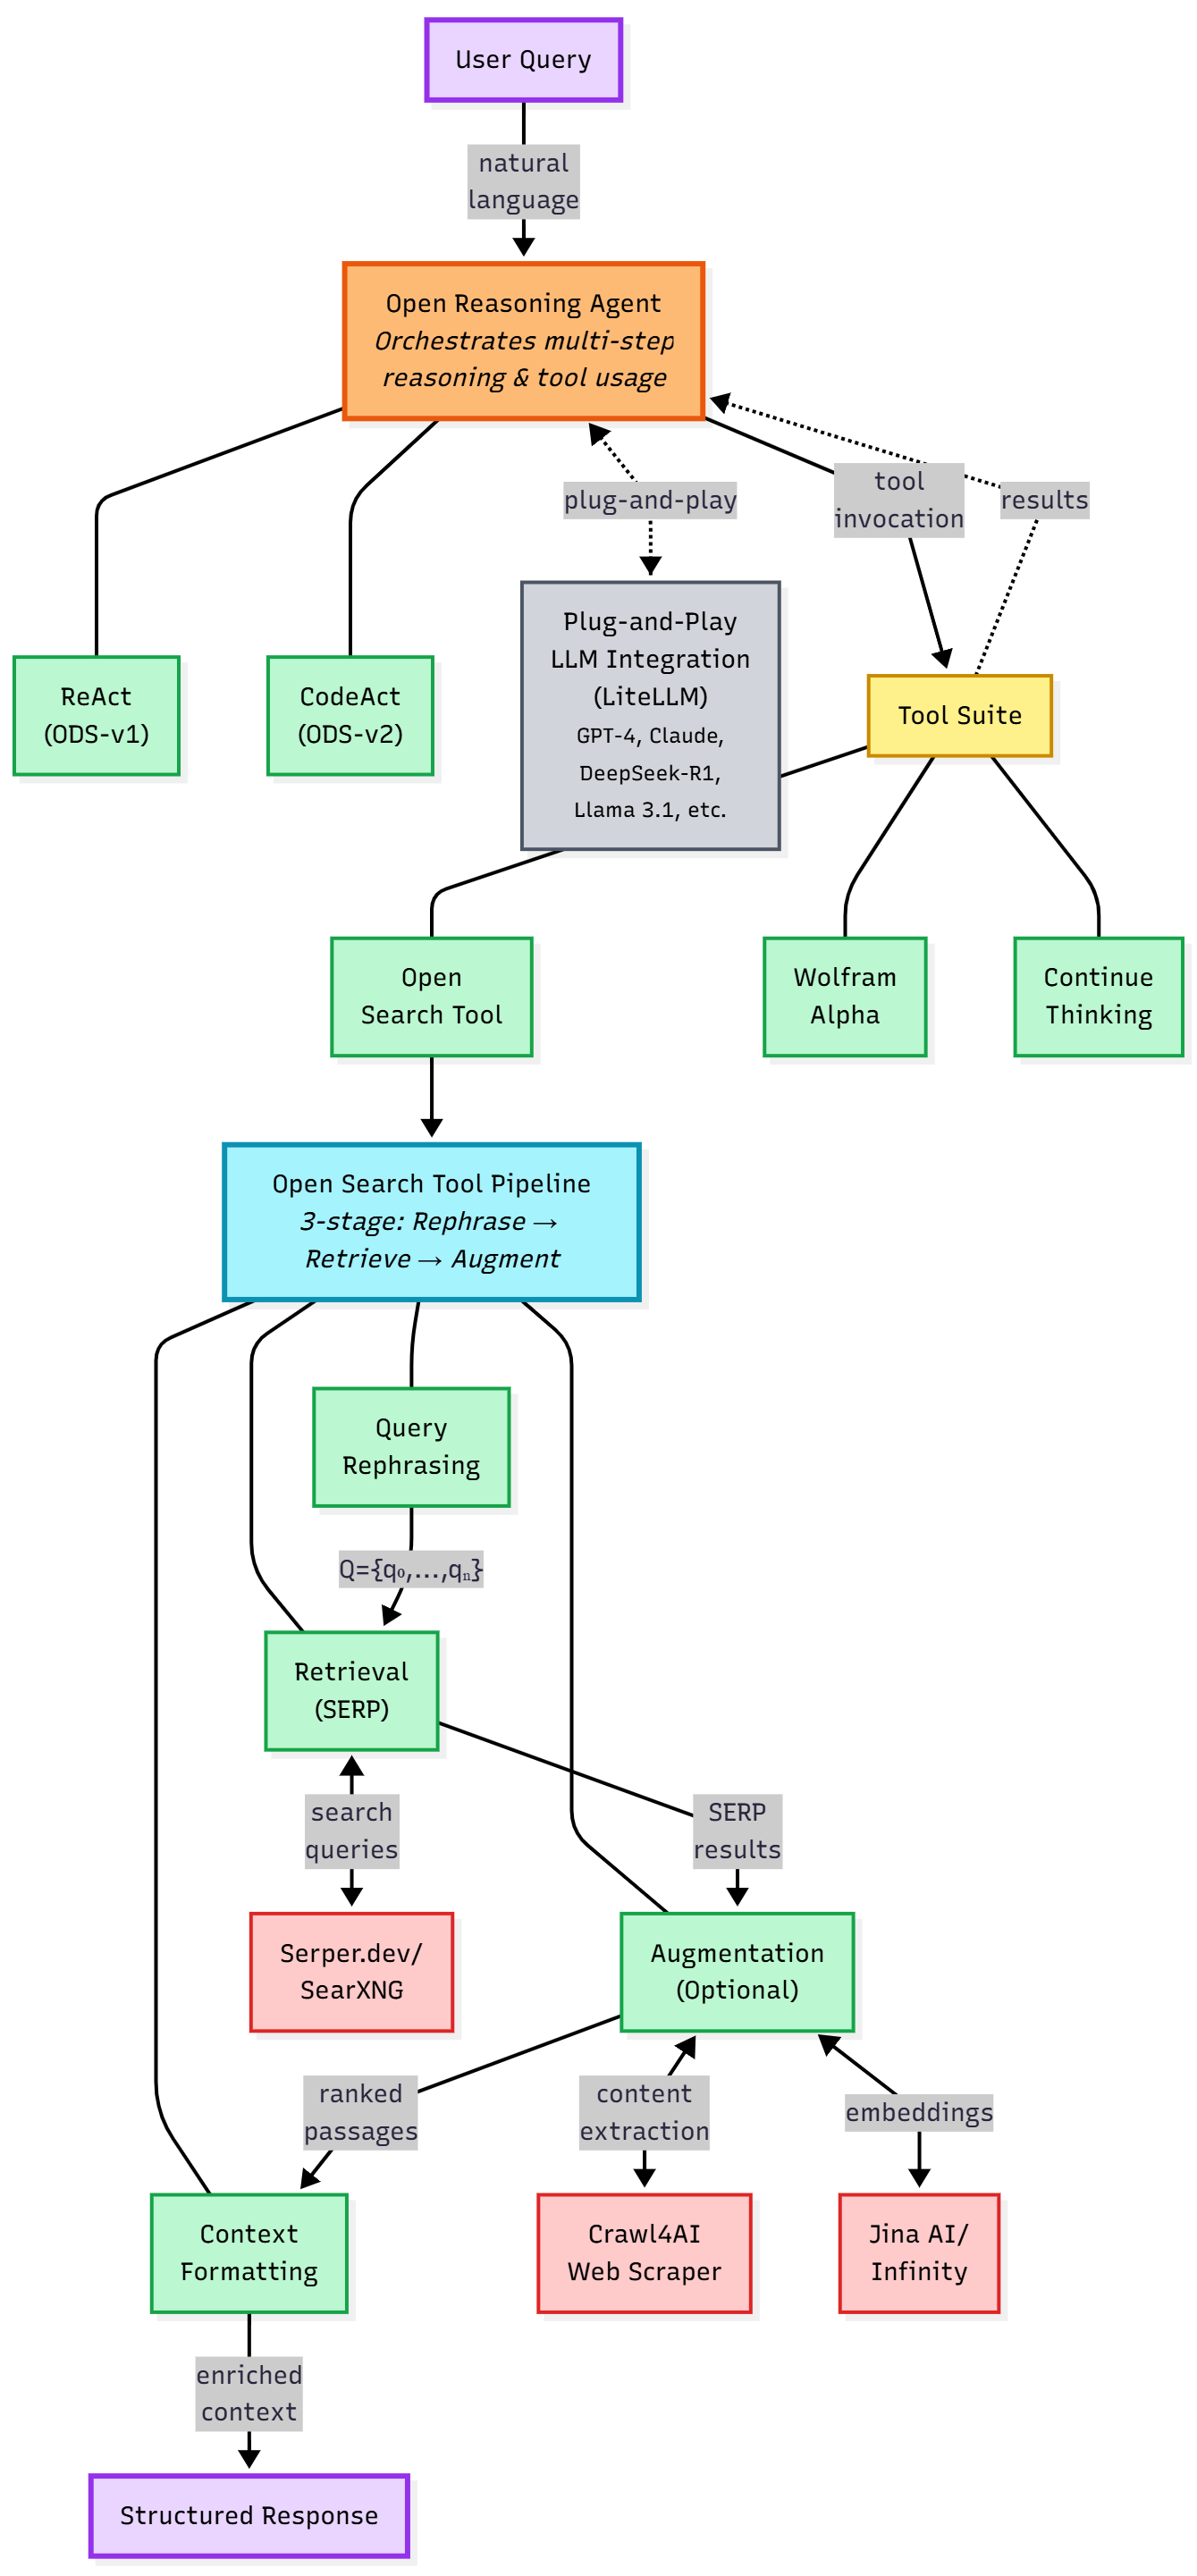
\includegraphics[width=0.5\linewidth]{figure1.png}
    \caption{Open Deep Search Two-Component Architecture. The system separates the Open Reasoning Agent (top) from the Open Search Tool (bottom), enabling independent optimization and flexible deployment. The agent orchestrates query resolution through iterative tool invocation, while the search pipeline transforms queries into rich contextual information through rephrasing, retrieval, and optional augmentation.}
    \label{fig:open_deep_search_architecture}
\end{figure}


\subsection{Dual Agent Framework: ODS-v1 and ODS-v2}

A distinctive characteristic of Open Deep Search is the provision of two complete agent implementations embodying different reasoning paradigms. Rather than selecting a single approach and optimizing exclusively for that pattern, the system offers both ReAct-based and CodeAct-based agents, enabling users to select the framework best suited to their requirements. This dual approach reflects empirical findings that different reasoning paradigms excel at different categories of tasks.

Open Deep Search version 1, denoted ODS-v1, implements the ReAct agent framework that combines reasoning and acting in an explicit loop structure. The agent operates by iterating through thought-action-observation cycles where each iteration begins with a thought that articulates the agent's current understanding and reasoning about how to proceed. The thought leads to an action representing a concrete step such as invoking the search tool with a specific query, performing a calculation, or continuing reasoning about a complex problem. The action produces an observation capturing the results of that action, such as search results from the web or the output of a mathematical computation. This observation feeds into the next thought, creating a feedback loop that progressively works toward query resolution.

The ReAct paradigm offers significant advantages in interpretability and control. The explicit thought traces provide human-readable explanations of the agent's reasoning process, facilitating debugging when the system produces incorrect results and building user trust through transparency. The structured format with distinct thought, action, and observation phases makes it straightforward to analyze system behavior and identify specific points where reasoning diverges from desired patterns. The framework naturally accommodates dynamic few-shot learning where relevant examples can be selected and included in prompts to guide the agent toward productive reasoning patterns. Open Deep Search implements this through a collection of 200 community-designed ReAct examples that demonstrate diverse reasoning approaches across different query types.

Open Deep Search version 2, denoted ODS-v2, implements the CodeAct agent framework where the agent generates executable Python code to accomplish tasks rather than using structured natural language action specifications. When presented with a query, the ODS-v2 agent analyzes what steps are necessary and produces Python code that invokes appropriate tools, processes results, and synthesizes answers. The generated code executes within a controlled environment that provides access to registered tools including the Open Search Tool, mathematical computation capabilities, and any additional tools configured for the deployment.

The CodeAct paradigm provides distinct advantages particularly for complex multi-step reasoning tasks. Programming languages naturally express composition where the output of one operation feeds as input to another, making it easier to chain multiple search operations and process results programmatically. Code provides better abstraction mechanisms including variables, functions, and control flow constructs that simplify expression of complex reasoning patterns. The paradigm enables more sophisticated error handling where the generated code can include exception handling, retry logic, and alternative pathways that improve robustness. The format allows agents to maintain state across reasoning steps more naturally than the structured ReAct format, which proves valuable for queries requiring accumulation of information across multiple searches.

Empirical performance data demonstrates that these different reasoning paradigms excel in different scenarios. On the SimpleQA benchmark comprising relatively straightforward factual queries, both approaches perform similarly. Open Deep Search version 1 using Llama 3.1 70B achieves 83.4 percent accuracy while version 2 achieves 83.6 percent, a negligible difference. However, on the FRAMES benchmark testing complex multi-hop reasoning, the performance gap becomes substantial. Using DeepSeek-R1 as the base model, ODS-v1 achieves 56.7 percent accuracy while ODS-v2 reaches 75.3 percent, an 18.6 percentage point improvement. This performance differential suggests that the enhanced compositional capabilities and flexible control flow of code-based reasoning provide significant advantages for complex tasks requiring multiple search iterations and sophisticated information synthesis.

The architectural decision to support both agent frameworks rather than selecting a single approach reflects a pragmatic acknowledgment that no universal best solution exists across all use cases. Users deploying Open Deep Search for straightforward question answering where interpretability is paramount may prefer ODS-v1 with its explicit reasoning traces. Those addressing complex research tasks where maximum performance on multi-hop queries is essential may prefer ODS-v2 despite somewhat reduced interpretability of generated code. The availability of both options within a unified framework enables users to select the appropriate tool for their specific requirements without needing to adopt entirely different systems.

\subsection{Plug-and-Play Model Integration}

The model-agnostic architecture of Open Deep Search represents a strategic design decision that distinguishes it from systems optimized for specific language models. Rather than tightly coupling system capabilities to a particular model family, Open Deep Search provides a flexible integration framework that accommodates any model accessible through the LiteLLM unified interface. This design enables seamless integration with open-source models including Llama, DeepSeek, Qwen, Mistral, and others, as well as closed-source models accessed via API including GPT-4, Claude, Gemini, and additional alternatives.

The integration mechanism operates through a simple configuration pattern where users specify model identifiers and API credentials through environment variables. The system handles all details of model communication including request formatting, response parsing, error handling, and retry logic. This abstraction shields users from the complexities of interfacing with diverse model providers, each of which implements different API conventions, authentication mechanisms, and response formats. The LiteLLM library provides the foundation for this unified interface, supporting over fifty different model providers and hundreds of specific models.

The plug-and-play architecture provides several important benefits for different stakeholder groups. Researchers benefit from the ability to conduct comparative studies across different base models to understand how model capabilities affect overall system performance. The architecture enables controlled experiments where the search tool and reasoning framework remain constant while only the underlying language model changes, isolating the effect of model selection on outcomes. This facilitates research on questions such as how model size affects search-augmented reasoning, whether models specifically trained for reasoning tasks provide advantages over general-purpose models, and how different model families with varying architectural choices compare on search-intensive tasks.

Practitioners deploying Open Deep Search for production applications benefit from flexibility in navigating trade-offs between performance, cost, latency, and privacy. Users with strict latency requirements can select faster models that generate responses more quickly even if they sacrifice some accuracy. Cost-sensitive deployments can choose more economical models that provide acceptable performance at lower price points. Privacy-conscious applications can deploy self-hosted open-source models that process queries entirely within private infrastructure without sending data to external API providers. As new models become available with improved capabilities or more favorable cost-latency-performance trade-offs, users can adopt them immediately without requiring system modifications or retraining.

The architecture also provides a natural pathway for capability improvement over time. As the field of language model development continues rapid advancement, state-of-the-art capabilities regularly shift between different model families and providers. A system tightly coupled to a specific model risks obsolescence as better alternatives emerge. The plug-and-play architecture of Open Deep Search ensures that the system automatically benefits from progress in base model development. Empirical data demonstrates this effect clearly. Using Llama 3.1 70B as the base model, ODS-v1 achieves 83.4 percent on SimpleQA. Switching to the more capable DeepSeek-R1 while keeping all other components identical improves performance to 87.7 percent, a gain of 4.3 percentage points solely from improved base model capabilities. This demonstrates that Open Deep Search successfully leverages improvements in foundation models without requiring architectural changes.

The model-agnostic design also facilitates domain specialization where different models optimized for specific domains can be deployed for applications in those areas. Medical applications might benefit from biomedical language models trained on scientific literature and clinical notes. Legal applications could leverage models trained on case law and legal documents. Financial applications might deploy models with enhanced capabilities for numerical reasoning and economic analysis. The Open Deep Search architecture accommodates all such specializations through the same integration framework, requiring only that the specialized model be accessible through a supported API provider.

Certain technical considerations arise from the decision to support arbitrary model integration. Different models have varying context window limits that constrain how much search result context can be provided in a single query. The system must adapt to these limits by truncating or summarizing context when necessary, potentially affecting performance for queries requiring substantial background information. Models differ in their instruction-following capabilities, with some models requiring careful prompt engineering to reliably follow the structured formats expected by ReAct or CodeAct agents. The system addresses this through flexible prompt templates that can be customized for different model families. Models vary in their tool-use capabilities, with some having been specifically trained for function calling while others require learning tool usage patterns from few-shot examples. The architecture accommodates this variation through configurable few-shot example selection and prompt templates tailored to model capabilities.

Despite these considerations, the plug-and-play architecture successfully abstracts over model-specific details while providing a unified interface for search-augmented reasoning. The design demonstrates that effective integration across diverse models is achievable without sacrificing the benefits of modularity and flexibility that make open systems valuable for research and practical deployment.

\subsection{Operational Modes and Deployment Flexibility}

Open Deep Search provides two distinct operational modes that present different trade-offs between latency and accuracy, enabling users to select the appropriate configuration for their specific use case and performance requirements. This flexibility acknowledges that different applications have varying priorities regarding response time versus answer quality.

Default mode optimizes for rapid response generation by limiting the depth of information processing. In this mode, the Open Search Tool executes query rephrasing and retrieval but skips the augmentation stage that involves web scraping, content extraction, and semantic reranking. The system relies exclusively on search engine result page snippets rather than fetching and processing full webpage content. This approach significantly reduces latency by eliminating the time required for multiple web requests, content parsing, and embedding generation. Default mode proves well-suited for queries where search engine snippets provide sufficient context, applications where response time is critical, and deployments operating under tight computational budgets.

Pro mode prioritizes accuracy and comprehensiveness by enabling the complete augmentation pipeline. After retrieving search engine result pages, the system proceeds to scrape full content from top-ranked URLs, break that content into semantic chunks, generate embeddings for relevance assessment, rerank chunks based on their semantic similarity to the query, and incorporate the highest-scoring passages into context provided to the reasoning agent. This additional processing substantially increases the amount and quality of information available for answer generation. Pro mode excels for complex multi-hop queries requiring synthesis across multiple sources, research applications where accuracy is paramount, and scenarios where users are willing to accept longer response times in exchange for more comprehensive answers.

Empirical performance data quantifies the trade-off between these modes. On the FRAMES benchmark, Open Deep Search version 2 using DeepSeek-R1 achieves 75.3 percent accuracy in pro mode with augmentation enabled. Disabling augmentation and operating in default mode reduces accuracy to 27.6 percent, a dramatic decline of 47.7 percentage points. This demonstrates that augmentation is essential for complex reasoning tasks where search engine snippets alone prove insufficient. However, the latency characteristics differ substantially. Default mode typically completes queries in five to fifteen seconds depending on the number of search iterations required. Pro mode extends this to fifteen to sixty seconds due to web scraping and embedding generation overhead. This represents a four-fold increase in latency in exchange for nearly three-fold improvement in accuracy on complex tasks.

The architectural support for operational mode selection extends beyond simply enabling or disabling augmentation. The system provides fine-grained control over multiple parameters that affect the performance-latency trade-off. Users can configure the number of URLs to scrape during augmentation, balancing between comprehensive coverage requiring more time and focused analysis of top results. The maximum number of search iterations can be limited for latency-sensitive applications or left unbounded for exhaustive research queries. Temperature parameters controlling language model randomness can be adjusted to trade between creative exploration and focused retrieval of known facts. Context window utilization can be configured to include more or fewer search results based on available model context capacity.

This flexibility enables sophisticated deployment patterns where different operational modes serve different user populations or query types within a single system. A production deployment might implement tiered service levels where basic users receive default mode processing with rapid response times while premium subscribers access pro mode with enhanced accuracy. The system could implement adaptive mode selection where simple queries detected through heuristic classification automatically use default mode while complex queries trigger pro mode processing. Interactive applications might begin with default mode to provide rapid initial responses and then optionally refine answers using pro mode if users indicate the initial response was insufficient.

The deployment flexibility extends to infrastructure choices where users can select between cloud-based API usage for convenience, self-hosted deployments for privacy and cost optimization at scale, and hybrid configurations that use self-hosted components for sensitive operations while leveraging cloud APIs for computationally intensive tasks. This flexibility acknowledges that different organizations have varying requirements regarding data privacy, cost structures, operational expertise, and performance priorities. The modular architecture ensures that these deployment variations remain possible without requiring fundamental system redesign.

\subsection{Integration Points and Extensibility}

The architecture of Open Deep Search deliberately exposes integration points that enable extension of system capabilities beyond the core search and reasoning components provided in the base implementation. This extensibility serves multiple purposes including customization for domain-specific applications, integration into larger system architectures, and experimentation with novel capabilities by researchers.

The tool integration framework represents the primary extension mechanism for adding new capabilities to the reasoning agents. Both ODS-v1 and ODS-v2 support registration of arbitrary tools that the agent can invoke during query processing. The base system includes three tools comprising the Open Search Tool for web search, Wolfram Alpha integration for mathematical computation, and a continue thinking tool that enables recursive reasoning about complex problems. However, the framework accepts any tool implementing the required interface that takes string inputs and returns string outputs. This simple contract enables integration of diverse capabilities including database queries for structured data access, API calls to external services for real-time information, code execution environments for programming tasks, and specialized knowledge bases for domain expertise.

Domain-specific deployments can leverage this extensibility to incorporate specialized tools relevant to their applications. A medical deployment might add tools for querying PubMed, accessing clinical trial databases, and looking up drug interactions. A legal deployment could integrate case law databases, statute search capabilities, and legal citation verification. A financial application might include tools for retrieving stock prices, accessing SEC filings, and performing financial calculations. The reasoning agents treat these specialized tools identically to the core search capability, invoking them when relevant to query resolution and incorporating results into their reasoning process.

The search provider abstraction enables integration with alternative search backends beyond the default Serper and SearXNG options. Organizations with existing search infrastructure can implement the search provider interface to integrate their internal systems. Specialized deployments might incorporate domain-specific search engines such as Google Scholar for academic queries, GitHub search for code-related questions, or social media APIs for trend analysis. The modular architecture ensures that changing search providers requires no modifications to reasoning agents or other system components.

The reranking interface provides another extension point where alternative embedding models and semantic similarity approaches can be integrated. While the base system supports Jina AI cloud-based reranking and self-hosted Infinity servers, the interface accepts any implementation that can score passage relevance to queries. Researchers experimenting with novel reranking approaches can integrate them seamlessly. Domain-specific deployments might use specialized embedding models trained on relevant corpora to improve retrieval quality for their particular domains.

The prompt template system enables customization of how agents interact with base language models without modifying core system code. Templates define the structure of prompts including system messages, few-shot examples, and formatting conventions. Users can customize templates to improve performance with specific model families, incorporate domain-specific instructions, adjust the style and format of generated responses, and experiment with different prompting strategies. This flexibility proves particularly valuable given the diversity of language models with varying instruction-following characteristics and optimal prompt formats.

The integration points extend beyond individual components to system-level composition where Open Deep Search can operate as one element within larger multi-agent architectures. The Sentient Agent Framework provides orchestration capabilities for coordinating multiple specialized agents, each potentially running independent instances of Open Deep Search configured for different domains. The clean interfaces exposed by Open Deep Search components facilitate this integration where the search tool can be registered with external agent frameworks, reasoning agents can coordinate with agents implemented using different frameworks, and shared resources like caches and embeddings can be utilized across agent systems.

This extensibility reflects a design philosophy that views Open Deep Search not as a complete solution for all possible search and reasoning tasks but rather as a flexible foundation that users can adapt and extend to meet their specific requirements. The architecture provides substantial capabilities out of the box while ensuring that the extension mechanisms enable unlimited customization for specialized needs. This balance between functionality and flexibility positions Open Deep Search as both a production-ready system for common use cases and a research platform for exploring novel approaches to search-augmented reasoning.

\subsection{Architectural Design Decisions and Trade-offs}

Every architectural choice involves trade-offs between competing objectives. Understanding the specific trade-offs reflected in Open Deep Search design decisions provides insight into the system's strengths and limitations across different use cases and deployment scenarios.

The decision to implement two separate agent frameworks rather than selecting a single approach carries both benefits and costs. The dual framework approach enables users to select the reasoning paradigm best suited to their requirements, facilitates comparative research on reasoning approaches, and provides redundancy where one framework can serve as fallback when the other encounters difficulties. However, this approach increases implementation complexity by requiring maintenance of two agent codebases, complicates documentation and user education by presenting multiple options, and potentially fragments community contributions across different frameworks. The empirical performance differential on FRAMES benchmark suggests that the benefits outweigh costs by providing substantially better performance on complex tasks through CodeAct while maintaining interpretability through ReAct for simpler applications.

The query rephrasing component exemplifies trade-offs between search diversity and computational cost. Rephrasing expands a single user query into multiple related queries that improve coverage and recall of relevant information. This proves particularly valuable for ambiguous queries where the user's intent might map to multiple search formulations. However, rephrasing requires an additional language model call before search begins, adding latency and cost. The system must balance between generating too few rephrased queries that provide insufficient diversity and too many that waste resources on redundant searches. The implementation addresses this by dynamically generating between two and five rephrased queries based on query complexity, providing a reasonable balance for most use cases while remaining configurable for specific requirements.

The augmentation pipeline design reflects trade-offs between answer quality and response latency. Deep augmentation through web scraping and semantic reranking dramatically improves performance on complex multi-hop queries, as evidenced by the 47.7 percentage point improvement on FRAMES. However, this processing adds significant latency through multiple web requests, content parsing, embedding generation, and reranking computation. The architectural choice to make augmentation optional through default versus pro modes acknowledges that different applications have varying priorities on this trade-off. The system provides the flexibility to select the appropriate operating point rather than forcing a single choice on all users.

The plug-and-play model integration reflects a strategic choice to prioritize flexibility over optimization. An alternative approach would be to select a specific base model and optimize all components specifically for that model's characteristics including prompt engineering, context window utilization, and tool-use patterns. This optimization might yield somewhat better performance for the selected model. However, it would sacrifice the ability to easily adopt new models as they become available, limit users to a single model provider, and constrain deployment flexibility across different privacy and cost requirements. The trade-off evaluation suggests that the benefits of model agnosticism outweigh the marginal performance gains from model-specific optimization, particularly given the rapid pace of language model development where state-of-the-art capabilities shift frequently between model families.

The decision to maintain explicit separation between search and reasoning components rather than implementing an end-to-end system involves trade-offs between modularity and integration. The separation enables independent development and optimization of components, facilitates testing and debugging through isolation of functionality, and supports flexible deployment configurations. However, the interface between components creates potential inefficiencies where the reasoning agent cannot directly influence how the search tool executes queries beyond the query text itself, information cannot flow bidirectionally to refine search strategy based on preliminary results, and the clean separation might miss opportunities for joint optimization of search and reasoning. The architectural choice reflects a judgment that the benefits of modularity for development, research, and deployment flexibility outweigh the potential performance gains from tighter integration.

The provision of self-hosting capabilities alongside API-based deployment options reflects trade-offs between convenience and control. API-based deployment offers simplicity where users need only configure credentials to access cloud services, provides elastic scaling without infrastructure management, and eliminates operational overhead. However, it incurs ongoing costs that scale with usage, raises privacy concerns by sending queries to external providers, and creates dependence on external service availability. Self-hosting provides cost advantages at scale, complete privacy and data control, and independence from external services. However, it requires substantial operational expertise, involves upfront infrastructure investment, and places maintenance burden on deploying organizations. The architectural support for both options acknowledges that different users appropriately make different trade-offs on this dimension based on their specific circumstances.

These architectural decisions and their associated trade-offs reveal a design philosophy that prioritizes flexibility, transparency, and extensibility while accepting some costs in implementation complexity and potential suboptimality for specific narrow use cases. This philosophy aligns with the broader goals of open-source development where serving diverse community needs and enabling customization takes precedence over achieving maximum performance on a single benchmark or use case. The resulting architecture provides a robust foundation for search-augmented reasoning that different users can adapt to their particular requirements while maintaining compatibility with a common core system and community.
